\documentclass[12pt]{article}
\usepackage{minted}
\usepackage{graphicx}
\usepackage{mathtools}
\usepackage{amsfonts}

\begin{document}
    \title{CS 541 Homework 1}
    \author{Stephen Szemis}
    \date{September 27, 2020}
    \maketitle

    \paragraph{Problem 1: Random Projection for Nearest Neighbor Search} ~\\
    I wrote the following code in order to generate the data. See comments for
    explanation.
    \inputminted{python}{hw1.py}

    The data is shown below, since this data is generated randomly I've include 
    three different runs.
    \begin{center}
        

    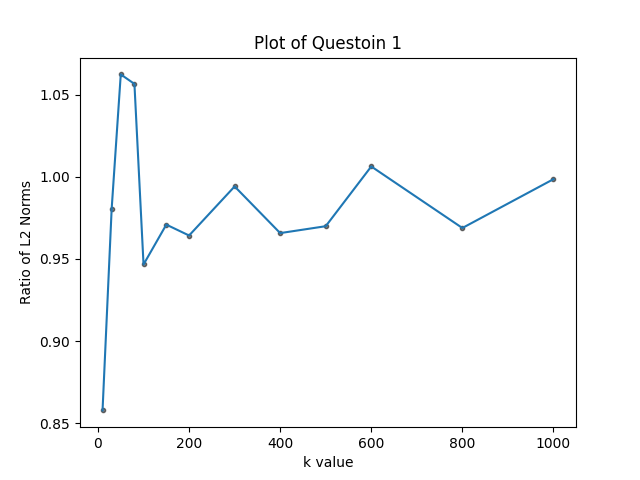
\includegraphics[width=10cm]{Figure_1.png}


    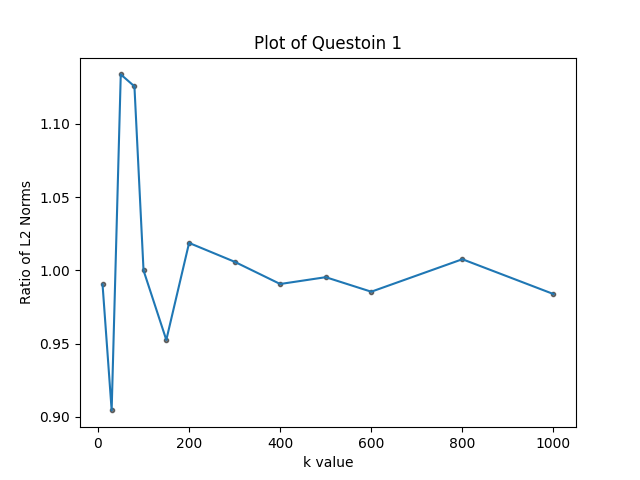
\includegraphics[width=10cm]{Figure_2.png}


    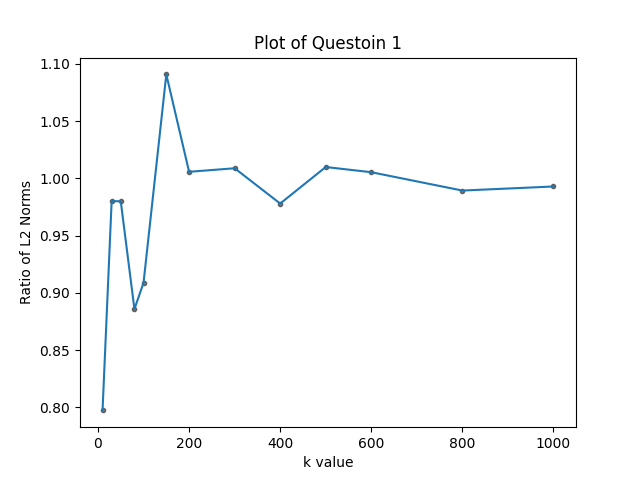
\includegraphics[width=10cm]{Figure_3.png}
    \end{center}

    As can be seen in the above graphs, the ratio between \(\|\textbf{x}\|\) and 
    \(\|\textbf{A}\|\) approach 1 sometime around \(k=200\). 
    This means that in general we can say that for some vector with 
    dimension \(d\), we can safely use random projection to lower it's dimension 
    by about \(1/5\) the size, while
    still keeping the distance between the data similar.

    \paragraph{Problem 2: Reliable Data Annotation}
    \begin{enumerate}
        \item The condition can be described like so\dots
        \[Pr(\sum_{i=1}^{n} y_i > 0)\]
        \item Chebyshelv's Inequality is written as\dots
        \[Pr(|X-\mathbb{E}[X]| \ge t) \le \frac{Var[X]}{t^2}\]
        Let \(X\) be our condition from part 1. We need the expected value and 
        variance of \(X\) for Chebyshelv's.
        \[
            \mathbb{E}[X] 
            = \mathbb{E} \left[ \sum_{i=1}^{n} y_i \right] 
            = \sum_{i=1}^{n} \mathbb{E} [y_i]
            = n * (0.6 - 0.4) = 0.2n
        \]
        \[
            Var[X] 
            = Var \left[ \sum_{i=1}^{n} y_i \right]
            = \sum_{i=1}^{n} Var[y_i]
            = n * (\mathbb{E}[y_i^2] - \mathbb{E}[y_i]^2)
            = 0.96n
        \]
        With that information we can now start calculating the inequality.
        \[
            Pr(|X - 0.2n| \ge t) \le \frac{0.96n}{t^2}
        \]
        Knowing we want a probability of 0.99 and X to be at least 1, we can write\dots
            \[0.2n - t = 1 \]
            \[\frac{0.96n}{t^2} = 0.01\]
        Solving the quadratic for n and t we find.
        \[ n \approx 2410 \]
        \[ t \approx 481 \]
        
        \item We will use the form of the Chernoff bound.
        \[
            Pr(Z \le (1 - \alpha)\mu n) \le e^{-\frac{\alpha^2 \mu n}{2}}    
        \]
        Our \(\mu = 0.6\). Note: Our condition was changed from part 1, since 
        we need to our random variables to be {0, 1} not {-1, 1}. Instead of looking for
        the sum to be greater then zero, we now look for the sum to be greater then half of 
        the total, or \(\frac{n}{2}\).
        Essentially we want the probability that Z is less then
        half of n to be lower then 1 percent. Written formally:
        \[ (1 - \alpha) 0.6n = \frac{n}{2}\]
        \[ e^{-\frac{\alpha^2 * 0.6n}{2}} = 0.01\]
        Solving for n and \(\alpha\) we get\dots
        \[
            \alpha = \frac{1}{6}
        \]
        \[
            -\frac{\alpha^2 * 0.6n}{2} = ln(0.01)
        \]
        \[
            n \approx 553
        \]
        \item In conclusion, it is easy to see from our estimates of n that the Chernoff bound gives a much 
        tighter approximation. This makes sense since it makes use of the inherent properties of the {0 ,1}
        distribution and therefore can get exponentiation on the right hand side of the probability.
    \end{enumerate}
\end{document}